\begin{enumerate}[\bfseries \textbf{Ejercicio} 1.]

%----------1.
\item \textbf{\boldmath Encontrar el punto final de $\vec{a}=(7,6)$ si el punto inicial es $P_0(2,-1)$.\\\\
    Respuesta.-}\; Sea $\vec{a}=P_1-P_0$ y $P_1=(x,y)$, entonces podemos hallar los vectores de la siguiente manera,
	$$x-2=7 \quad ; \quad y+1=6$$
    de donde $x=9, \; y=5$ y por lo tanto $$P_1=(9,5)$$\\

%----------2.
\item \textbf{\boldmath Sean $\vec{u}=(1,3)$,  $\vec{v}=(2,1)$ y $\vec{w}=(4,-1)$. Encontrar las componentes del vector $\vec{x}$ que satisfacen $2\vec{u}-\vec{v}+\vec{x}=7\vec{x}+\vec{w}$.\\\\
    Respuesta.-}\; Despejando $\vec{x}$ obtenemos $$6\vec{x}=2\vec{u}-\vec{v}-\vec{w} \quad \Rightarrow\quad 6\vec{x}=(2,6)-(2,1)-(4,-1)$$ 
    de donde $$6\vec{x}=(0,5)-(4,-1)\quad \Rightarrow \quad 6\vec{x}=(-4,6) \quad \Rightarrow \quad \vec{x}=\left(-\dfrac{2}{3},1\right)$$\\

%----------3.
\item \textbf{\boldmath Demuéstrese que: $0\vec{x}=\vec{0}$ y $r\vec{0}=\vec{0}$.\\\\
    Demostración.-}\; sea $\vec{x}\in V_n$ entonces $0\vec{x}=0(x_1,x_2,...,x_n)$, luego por la multiplicación de un número real por un vector tenemos, $$0\vec{x}=(0\cdot x_1,0\cdot x_2,...,0\cdot x_n)=(0,0,...,0)$$
    y por lo tanto se demuestra que $0\vec{x}=\vec{0}.$ Por otro lado sea $r\in \mathbb{R}$, por lo tanto $$r\vec{0}=r(0,0,...,0)=(r\cdot 0,r\cdot 0,...,r\cdot)=(0,0,...,0)$$
    de modo que $$r\vec{0}=\vec{0}$$\\

%----------4.
\item \textbf{Demuéstrese que:}
\begin{enumerate}[\bfseries a)]

    %-----a)
    \item \textbf{\boldmath Si $\vec{a}+\vec{b}=\vec{a}+\vec{c} \quad \Rightarrow \quad \vec{b}=\vec{c}$.\\\\
	Demostración.-}\; Sea $\vec{a},\vec{b},\vec{c} \in V_n$, entonces por el inverso aditivo e hipótesis tenemos ,
	\begin{center}
	    \begin{tabular}{rcl|l}
		$\vec{b}$&$=$&$(\vec{b}+\vec{a})-\vec{a}$&\\
			 &$=$&$(\vec{a}+\vec{b})-\vec{a}$&\\
			 &$=$&$(\vec{a}+\vec{c})-\vec{a}$&$\vec{a}+\vec{b}=\vec{a}+\vec{c}$\\
			 &$=$&$\vec{c}+(\vec{a}-\vec{a})$&\\
		&$=$&$\vec{c}$\\\\
	    \end{tabular}
	\end{center}
	\vspace{0.5cm}

    %-----b)
    \item \textbf{\boldmath Si $r\vec{x}=\vec{0}\quad \Rightarrow \quad r=0 \lor \vec{x}=\vec{0}$.\\\\
	Demostración.-}\; Será lo mismo demostrar $r\vec{x}=\vec{0}  \land r\neq 0\;\Rightarrow\;\vec{x}=\vec{0}$.\\ 

	Sea $r\in \mathbb{R}$ y $\vec{x} \in V_n$, entonces $$r\vec{x}=0 \;\; \mbox{implica que}\;\;  \vec{x}=\dfrac{\vec{0}}{r}, \;\; \mbox{ya que}\;\; r\neq 0.$$ Luego se sigue que $$\vec{x}=\vec{0}$$\\

    %-----c)
    \item \textbf{\boldmath Si $r\vec{x}=s\vec{x}\;\land\; \vec{x}\neq 0 \quad \Rightarrow \quad r=s$.\\\\
	Demostración.-}\; Reescribiendo se tiene: Si $r\vec{x}=s\vec{x}\; \land \; r\neq s \;\; \Rightarrow \; \; \vec{x}=0$.\\\\ 
	De donde se tiene $$\vec{x}=(r-s)\vec{x} \; \Rightarrow \; \vec{x}=r\vec{x}-s\vec{x} \; \; \mbox{ya que }\; r\neq s,$$ 
	por lo tanto $$\vec{x}=r(\vec{x}-\vec{x}).$$
	Aplicando la unicidad y existencia del inverso aditivo, se sigue 
	$$\vec{x}=r(0) \; \Rightarrow \; \vec{x}=0.$$\\

\end{enumerate}

%----------5.
\item \textbf{\boldmath Demostrar que si $\vec{c}\neq 0$ y si $\vec{a}$ y $\vec{b}$ son paralelos a $\vec{c}$, entonces $\vec{a}$ y $\vec{b}$ son paralelos. (Vectores paralelos a un mismo vector no nulo son paralelos entre sí).\\\\
    Demostración.-}\; Sea $\vec{a},\vec{b},\vec{c}\in V_n$. Por definición de vectores paralelos se tiene $$r_1\vec{a}=\vec{c}\quad \mbox{y} \quad r_2\vec{b}=\vec{c}$$ de donde $$r_1\vec{a}=r_2\vec{b},$$ en vista de que $r_1\cdot r_2 \neq 0$ entonces $$\vec{b}=r_1r_2^{-1} \vec{a},$$ por lo tanto se concluye que $\vec{a}$ y $\vec{b}$ son paralelos entre sí.\\\\

%----------6.
\item \textbf{\boldmath Hallar todos los vectores ortogonales a:}
\begin{enumerate}[\bfseries a)]
    
    %-----a)
    \item \textbf{\boldmath $(3,6)$\\\\
	Respuesta.-}\; Sea $(r_1,r_1)$ un vector, entonces para hallar vectores paralelos a $(3,6)$ utilizamos la definición como sigue,
	\begin{center}	
	    \begin{tabular}{rcr}
		$(3,6)\circ (r_1,r_2)$&$=$&$0$\\
		$3r_1+6r_2$&$=$&$0$\\
		$3(r_1+2r_2)$&$=$&$0$\\
		$r_1+2r_2$&$=$&$0$\\
		$r_1$&$=$&$-2r_2$\\
	    \end{tabular}
	\end{center}
	de donde tomamos valores para $r_2$, reemplazamos en (1) y obtendremos $n$ vectores paralelos a $(3,6)$.\\\\

    %-----b)
    \item  \textbf{\boldmath $(2,-1)$.\\\\
	Respuesta.-}\; Análogamente al inciso a) tenemos 
	\begin{center}
	\begin{tabular}{rcl}
	    $(2,-1)\circ (r_1,r_2)$&$=$&$0$\\
	    $2r_1 + (-r_2)$&$=$&$0$\\
	    $r_1$&$=$&$\frac{1}{2}r_2$\\
	\end{tabular}
	\end{center}
	de igual forma al anterior inciso, tomamos valores para $r_2$, y hallamos $n$ valores ortogonales a $(2,-1)$.\\\\

    %-----c)
    \item \textbf{\boldmath $(2,3,-1)$\\\\
	Respuesta.-}\; Sea $(r_1,r_2,r_3)$ un vector en $V_3$, entonces, 
	\begin{center}
	\begin{tabular}{rcl}
	    $(2,3,-1)\circ (r_1,r_2,r_3)$&$=$&$0$\\
	    $2r_1+3r_2-r_3$&$=$&$0$\\
	    $r_1$&$=$&$(r_3-3r_2)/2 \qquad$ (1)\\
	\end{tabular}
	\end{center}
	luego reemplazamos valores a $r_3$ y $r_2$ en (1), de donde obtendremos vectores ortogonales a $(2,3,-1)$.\\\\

    %-----d)
    \item \textbf{\boldmath $(a_1,a_2)$\\\\
	Respuesta.-}\; Análogo a los anteriores incisos se tiene,
	    $$(a_1,a_2)\circ (r_1,r_2)=0 \quad \Rightarrow \quad 
	    a_1r_1 + a_2r_2=0 \quad \Rightarrow \quad
	    \left\{ \begin{array}{l} a_1=-a_2r_2/r_1 \\ a_2=-a_1r_1/r_2 \\ r_1=-a_2r_2/a_1 \\ r_2=-a_1r_1/a_1 \end{array}\right.$$

	    \vspace{.6cm}

\end{enumerate}

%----------7.
\item \textbf{\boldmath Encontrar un vector que sea ortogonal tanto a $\vec{u}$ como a $\vec{v}$.}
\begin{enumerate}[\bfseries a)]

    %-----a)
    \item \textbf{\boldmath $\vec{u}=-7i+3j+k, \quad \vec{v}=2i+4k$.\\\\
	Respuesta.-}
	$$\begin{array}{rcl}
	    \vec{u}\times \vec{v} &=& \left|\begin{array}{ccc}
	    i&j&k\\
	    7&3&1\\
	    2&0&4\\
	    \end{array}\right|=\left|\begin{array}{cc}3&1\\ 0&4 \end{array}\right|i - \left|\begin{array}{cc} 7&1\\2&4 \end{array}\right|j + \left|\begin{array}{cc} 7&3\\2&0 \end{array}\right|k\\\\
			      &=&(3\cdot 4 - 1\cdot 0)i - (7\cdot 4-2\cdot 1)j+(7\cdot 0 - 3\cdot 2)k.
    \end{array}$$
	Por lo tanto el vector que deseamos encontrar es $$\vec{u}\times \vec{v}=(12,-26,-6)$$\\

    %-----b)
    \item \textbf{\boldmath $\vec{u}=(-1,-1,-1), \quad \vec{v}=(2,0,2)$\\\\
	Respuesta.-}\;
	$$\vec{u}\times \vec{v} = \left|\begin{array}{rrr}
	    i&j&k\\
	    -1&-1&-1\\
	    2&0&2\\
	\end{array}\right|$$
	de donde $$\vec{u}\times \vec{v} = -2i +2k = (-2,0,2)$$\\

\end{enumerate}

%----------8.
\item \textbf{\boldmath Encontrar todos los vectores posibles de longitud $1$ ortogonales tanto a $\vec{a}=(3,-2,1)$ como a $\vec{b}=(-2,1,-3)$.\\\\
    Respuesta.-}\; Partamos encontrando el producto vectorial de los vectores $\vec{a}$ y $\vec{b}.$ 

    $$\vec{a}\times \vec{b} = \left|\begin{array}{rrr}
	i&j&k\\
	3&-2&1\\
	-2&1&-3\\
    \end{array}\right|=5i+7j-k=(5,7,-1).$$

    Esto nos garantiza que el vector $\vec{a}\times \vec{b}$ es ortogonal tanto a $\vec{a}$, como a $\vec{b}$. Luego podemos encontrar cualquier vector de longitud $1$ dividiendo el vector por su modulo. Es decir, 
    $$\dfrac{\vec{a}\times \vec{b}}{\|\vec{a}\times \vec{b}\|}=1.$$ 
    de donde, $$\dfrac{\vec{a}\times \vec{b}}{|\vec{a}\times \vec{b}|}=\dfrac{(5,7,-1)}{\sqrt{5^2+7^2+1^2}} = \dfrac{(5,7,-1)}{5\sqrt{3}} = \left(\dfrac{1}{\sqrt{3}},\dfrac{7}{5\sqrt{3}},-\dfrac{1}{5\sqrt{3}}\right).$$
    Por lo tanto los vectores de longitud $1$ ortogonales a $\vec{a}$ y $\vec{b}$, son $$\left(\dfrac{1}{\sqrt{3}},\dfrac{7}{5\sqrt{3}},-\dfrac{1}{5\sqrt{3}}\right) \qquad \mbox{y}\qquad \left(-\dfrac{1}{\sqrt{3}},-\dfrac{7}{5\sqrt{3}},\dfrac{1}{5\sqrt{3}}\right)$$
    El segundo vector cumple con la condición, ya que es el vector contrario a $\left(\dfrac{1}{\sqrt{3}},\dfrac{7}{5\sqrt{3}},-\dfrac{1}{5\sqrt{3}}\right)$.\\\\

%----------9.
\item \textbf{\boldmath Sean $\vec{a}=ti + j$ y $\vec{b}=4i+3j$. Encontrar el valor de $t$ tal que }

\begin{enumerate}[\bfseries a)]
    
    %-----a)
    \item \textbf{\boldmath $\vec{a}$ y $\vec{b}$ sean ortogonales.\\\\
	Respuesta.-}\; Sea $\vec{a}=ti + j=(t,1)$ y $\vec{b}=4i+3j=(4,3)$, entonces por definición de ortogonalidad tenemos 
	$$\vec{a}\circ \vec{b} = 0 \;\; \Rightarrow \; \; 4t+3=0 \;\; \Rightarrow \; \; t=-3/4$$\\

    %-----b)
    \item \textbf{\boldmath El ángulo entre $\vec{a}$ y $\vec{b}$ sea $\pi/4$.\\\\
	Respuesta.-}\; Aplicando $\vec{a}\circ \vec{b}=|\vec{a}||\vec{b}|\cos(\pi/4)$ tenemos, 
	$$4t+3=\sqrt{t^2+1}\cdot \sqrt{25}\cdot \dfrac{\sqrt{2}}{2} \;\; \Rightarrow \; \; (4t^2+3)^2=(t^2+1)\cdot\dfrac{25}{2}\cdot \dfrac{1}{2}$$
	de donde,  $$7t^2+48-7=0.$$
	Por lo tanto, $$t=\dfrac{1}{7} \quad \mbox{o}\quad t=-7$$\\

    %-----c)
    \item \textbf{\boldmath El ángulo entre $\vec{a}$ y $\vec{b}$ sea $\pi/6$.\\\\
	Respuesta.-}\; Análoga al anterior ejercicio tenemos $$4t+3=\sqrt{t^2+1}\cdot \sqrt{25}\cdot \dfrac{\sqrt{3}}{2}\;\; \Rightarrow \; \; (4t^2+3)^2=(t^2+1)\cdot\dfrac{25}{2}\cdot \dfrac{3}{4}\;\; \Rightarrow \; \; -11t^2+96t-39=0$$
	de donde $$t=\dfrac{48+25\sqrt{3}}{11} \quad \mbox{o} \quad t=\dfrac{48-25\sqrt{3}}{11}$$\\

    %-----d)
    \item \textbf{\boldmath $\vec{a}$ y $\vec{b}$ sean paralelos.\\\\
	Respuesta.-}\; Sea $\vec{a}=(t,1)$ y $\vec{b}=(4,3)$ entonces por definición de vectores paralelos tenemos que $$\vec{a}=c\vec{b} \quad \Rightarrow \quad (t,1)=c(4,3) \quad \Rightarrow \quad (t,1)=(4c,3c)$$
	de donde $$t=4c \qquad \mbox{y} \qquad 1=3c$$
	por lo tanto $c=\dfrac{1}{3}$. Se sigue $$t=\dfrac{4}{3}$$\\

\end{enumerate}

%----------10. 
\item \textbf{\boldmath Los vectores $\vec{a}$ y $\vec{b}$ forman un ángulo de $60^\circ$ con $\|\vec{a}\|=5,$ $\|\vec{b}\|=8$. Determinar $||\vec{a}-\vec{b}\|$ y $\|\vec{a}+\vec{b}\|$.\\\\
    Respuesta.-}\; Sea $$\| \vec{a}\pm\vec{b}\|^2=\|a\|^2\|b\|^2 \pm 2\|\vec{a}\|\|\vec{b}\|\cos \theta$$  
    entonces se tiene, $$\|a\pm b\|^2 = 5^2 + 8^2 \pm 2\cdot 5\cdot 8 \cos\left(60\cdot\dfrac{\pi}{180}\right)$$
    por lo tanto $$\|\vec{a}-\vec{b}\| = 7 \qquad y \qquad \|\vec{a}+\vec{b}\| = \sqrt{129}$$\\

%----------11.
\item \textbf{\boldmath Los vectores $\vec{a}$ y $\vec{b}$ forman un ángulo de $30^\circ$ con $\|\vec{a}\|=1$, $\|\vec{b}\|=\sqrt{3}$. Calcular el ángulo formado por los vectores $\vec{a}+\vec{b}, \vec{a}-\vec{b}$.\\\\
    Respuesta.-}\; Por el teorema de los cosenos, calculamos $$\|\vec{a}-\vec{b}\|^2 = 1^2 + \sqrt{3}^2 - 2\sqrt{3} \cos 30 = 4 \quad \Rightarrow \quad \|\vec{a}-\vec{b}\|=2.$$
    Luego calculamos el ángulo $\alpha$ asociado a $\vec{a}$ y $\vec{a}-\vec{b}$ de donde, 
    $$\cos\alpha = \dfrac{\|\vec{a}\|}{\|\vec{a}-\vec{b}\|} \quad \Rightarrow \quad \alpha =\arccos \left(\dfrac{\|\vec{a}\|}{\|\vec{a}-\vec{b}\|}\right) = \arccos\dfrac{1}{2}=\dfrac{\pi}{3}=60^\circ.$$
    Sea  $a+b$ la diagonal del paralelogramo formado por los lados $\vec{a}$ y $\vec{b}$ entonces, el ángulo de $a+b$ estará dado por $15^\circ$. Por lo tanto  $a+b$ y  $a-b$ forman un ángulo de, 
    $$180-60-15=105^\circ.$$\\

%----------12.
\item \textbf{\boldmath Dados dos vectores $\vec{a},\vec{b},\vec{c}$ que satisfacen la condición $\vec{a}+\vec{b}+\vec{c} = \vec{0}$ y sabiendo que $\|\vec{a}\|=3, \|\vec{b}\|=1,\|\vec{a}\|=4$. Calcular $\vec{a}\circ \vec{b}+\vec{b}\circ \vec{c}+\vec{a}\circ \vec{c}$\\\\
    Respuesta.-}\; Si $\vec{a}+\vec{b}+\vec{c}=0$ entonces $$0=\|\vec{0}\|^2=\|\vec{a}+\vec{b}+\vec{c}\|^2.$$ 
    Luego, 
    $$\begin{array}{rcl}
	0=\|\vec{a}+\vec{b}+\vec{c}\|^2 &=& \|\vec{a}+(\vec{b}+\vec{c})\|^2\\
				      &=& \|\vec{a}\|^2+2[\vec{a}\circ(\vec{b}+\vec{c})]+\|\vec{b}+\vec{c}\|^2\\
				      &=& \|\vec{a}\|^2+2\vec{a}\circ \vec{b}+2\vec{a}\circ \vec{b}+\|\vec{b}\|^2+2\vec{b}\circ \vec{c}+\|\vec{c}\|^2\\
				      &=& \|\vec{a}\|^2 + \|\vec{b}\|^2 + \|\vec{c}\|^2 + 2(\vec{a}\circ \vec{b} + \vec{a}\circ \vec{c} + \vec{b}\circ \vec{c}) 
    \end{array}$$
    Por lo tanto,
    $$\vec{a}\circ \vec{b} + \vec{a}\circ \vec{c} + \vec{b}\circ \vec{c} = -\dfrac{\|\vec{a}\|^2 + \|\vec{b}\|^2 + \|\vec{c}\|^2}{2} = -\dfrac{3^2+1^2+4^2}{2}=-13.$$\\


%----------13.
\item \textbf{\boldmath Dados los puntos $P(3,4)$, $Q(1,1)$ y $R(5,2)$, usar métodos vectoriales para encontrar las coordenadas del cuarto vértice del paralelogramo cuyo lados adyacentes son $\vec{PQ}$ y $\vec{QR}$.\\\\
    Respuesta.-}\; Grafiquemos la idea. 
    \begin{center}
	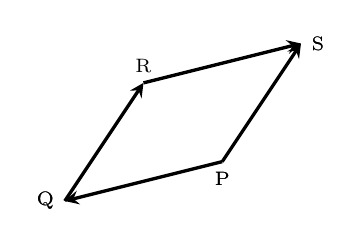
\begin{tikzpicture}[scale=.5]
	    \draw[line width=1.2pt,stealth-](3,4)node[above]{R}--(1,1)node[left]{Q};
	    \draw[line width=1.2pt,stealth-](1,1)node[left]{Q}--(5,2)node[below]{P};
	    \draw[line width=1.2pt,-stealth](5,2)node[below]{P}--(7,5)node[right]{S};
	    \draw[line width=1.2pt,stealth-](7,5)node[right]{S}--(3,4);
	\end{tikzpicture}
    \end{center}
    Sea $S$ el vértice a encontrar. Entonces, por las características de un paralelogramo tenemos 
    $$\vec{QR}=\vec{PS},$$ 
    por lo tanto $$(1-1)-(5,2)=(3,4)-S \quad \Rightarrow \quad S=(3,4)-(-4,-1)$$
    $$S=(7,5).$$\\


%----------14.
\item \textbf{\boldmath Demostrar que $(4,5,2),(4,7,9),(8,5,-6)$ son los vértices de un triángulo equilátero.\\\\
    Respuesta.-}\; Si $(4,5,2),(4,7,9),(8,5,-6)$ son los vértices de un triángulo equilátero, podemos hallar las longitudes de la siguiente manera: 

    $$\begin{array}{rcccccl}
	\|\vec{a}\| &=& \|(4,7,9)-(4,5,2)\|&=&\|(0,2,7)\| &=& \sqrt{53}.\\\\
	\|\vec{b}\| &=& \|(8,5,-6)-(4,7,9)\| &=& \|(4,-2,-15)\| &=& \sqrt{245}.\\\\
	\|\vec{c}\| &=& \|(8,5,-6)-(4,5,2)\| &=& \|(4,0,-8)\| &=& \sqrt{80}.\\\\
    \end{array}$$
    Luego, calculando el ángulo entre dos de los vectores encontrados, tenemos
    $$\cos(\theta)=\dfrac{\vec{a}\circ \vec{b}}{\|\vec{a}\|\|\vec{b}\|}=\dfrac{0\cdot 4 + 2\cdot(-2)+7\cdot(-15)}{\sqrt{53}\sqrt{245}}\quad \Rightarrow \quad \theta=\arccos\left(\dfrac{-109}{\sqrt{53}\sqrt{245}}\right)=163^\circ$$

    El cual contradice la proposición dada, ya que un triangulo equilatero tiene sus angulos igual a $60^\circ$.\\

    Podemos refutar la proposición dada de otra forma.\\
    Supongamos que las distancias entre $A,B$ y $C$ son iguales, lo que implica que 
    $$\|\vec{a}\|=\|\vec{b}\|=\|\vec{a}\|.$$ 
    Ya que $\|\vec{a}\|\neq \|\vec{b}\|$ se concluye que los puntos dado no son los vertices de un triangulo equilátero.\\\\


%----------15.
\item \textbf{\boldmath Demostrar que}
    \begin{enumerate}[a)]

	%---------- a)
	\item \textbf{\boldmath $(2,1,6), (4,7,9)$ y $(8,5,-6)$ son los vértices de un triángulo rectángulo.\\\\
	    Respuesta.-}\; Para demostrar que los puntos dados son vértices de un triángulo rectángulo, primero hallemos los vectores asociados, de la siguiente manera:
	    $$\begin{array}{rcccl}
		\vec{a} &=& (4,7,9)-(2,1,6) &=& (2,6,3)\\\\
		\vec{b} &=& (8,5,-6)-(4,7,9) &=& (4,-2,-15)\\\\
		\vec{c} &=& (8,5,-6)-(2,1,6) &=& (6,4,-12)\\
	    \end{array}$$
	    Luego, por definición de paralelismo de vectores, vemos que no existe un escalar $r\in \mathbb{Z}$ tal que 
	    $$\vec{a}=r\vec{b}.$$
	    Es decir,
	    $$\left\{\begin{array}{crr}
		    2&=&4r\\
		    1&=&-2r\\
		    6&=&-15r
		\end{array}\right. \quad \Rightarrow \quad
		\left\{\begin{array}{rcr}
		    r&=&\frac{1}{2}\\\\
		    r&=&-\frac{1}{2}\\\\
		    r&=&-\frac{6}{15}
		\end{array}\right.$$

	Así, podemos afirmar que los puntos dados corresponden a los vértices de un triángulo. Luego, para saber si este triángulo es rectángulo solo debemos hallar dos vectores ortogonales, como sigue:
	$$\vec{a}\circ \vec{c} =  (2,6,3)\circ (6,4,-12) = 2\cdot 6 + 6\cdot 4+3\cdot (-12) = 0$$
	Por lo tanto, los puntos dados son vértices de un triángulo rectángulo.\\\\

	%---------- b)
	\item \textbf{\boldmath ¿En cuál de los vértices está el ángulo de $90^\circ$?.\\\\
	    Respuesta.-}\; Se encuentra en el vértice $(2,1,6)$. Esto por el desarrollo del anterior ejercicio.\\\\

	%---------- c)
	\item \textbf{Encontrar el área del triángulo.\\\\
	    Respuesta.-}\; Se sabe que el área de un triángulo rectángulo es igual a la mitad del productos de sus catetos. Por lo tanto, el área del triángulo es igual a:
	    $$A=\dfrac{1}{2}\|\vec{a}\times \vec{c}\|$$
	    De donde,
	    $$\|\vec{a}\times \vec{c}\| = \| \left[ 6\cdot (-12)-3\cdot 4;3\cdot 6 - 2\cdot (-12);2\cdot 4 - 6\cdot 6\right]\| = \|-84,42,-28\| = 98.$$

	    Por lo tanto,
	    $$A=\dfrac{98}{2}=49.$$\\

    \end{enumerate}

%----------16.
\item \textbf{\boldmath Sean $\vec{a},\vec{b}\in \mathbb{R}$. Demuéstrese que $\|\vec{a}+\vec{b}\|^2-\|\vec{a}^2-\vec{b}\|^2=4\vec{a}\circ \vec{b}$.\\\\
    Demostración.-}\; Sabemos que 
    $$\|\vec{a}\pm \vec{b}\|^2=\|\vec{a}\|^2\pm 2\vec{a}\circ \vec{b}+\|\vec{b}\|^2$$
    Por lo tanto se tiene,
    $$\|\vec{a}+\vec{b}\|^2-\|\vec{a}^2-\vec{b}\|^2=|\vec{a}|^2 + 2\vec{a}\circ \vec{b} + | \vec{b} |^2 - \left(|\vec{a}|^2 - 2\vec{a} \circ \vec{b} + |\vec{b}^2|\right)=4\vec{a} \circ \vec{b}.$$\\

%----------17.
\item \textbf{\boldmath Demuéstrese que $\vec{a}+\vec{b}$ y $\vec{a}-\vec{b}$ son ortogonales si y sólo si $\|\vec{a}\|=\|\vec{b}\|.$ ¿Cuál es la interpretación geométrica del problema?.\\\\
    Demostración.-}\; 
    La interpretación geométrica viene dada por:
    \begin{center}
	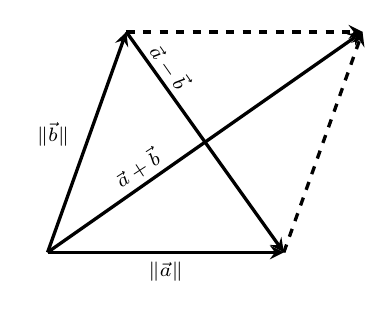
\begin{tikzpicture}[scale=1]
	    \draw[line width=1.2pt,-stealth](0,0)--(3,0);
	    \draw[dashed,line width=1.2pt,-stealth](1,2.8)--(4,2.8);
	    \draw[line width=1.2pt,-stealth](0,0)--(1,2.8);
	    \draw[dashed,line width=1.2pt,-stealth](3,0)--(4,2.8);
	    \draw[line width=1.2pt,-stealth](0,0)--(4,2.8);
	    \draw[line width=1.2pt,-stealth](1,2.8)--(3,0);
	    \draw(1.5,0)node[below]{$\|\vec{a}\|$};
	    \draw(.4,1.5)node[left]{$\|\vec{b}\|$};
	    \draw(1.5,1.3)node[left,rotate=33]{\scriptsize$\vec{a}+\vec{b}$};
	    \draw(1.8,2)node[left,rotate=-55]{\scriptsize$\vec{a}-\vec{b}$};
	\end{tikzpicture}
    \end{center}

    Por definición de vectores ortogonales tenemos que:
    $$\begin{array}{rcl}
	\left(\vec{a}+\vec{b}\right)\circ\left(\vec{a}-\vec{b}\right) = 0 &\Leftrightarrow&(\vec{a}+\vec{b})\circ \vec{a}+(\vec{a}+\vec{b})\circ (-\vec{b})\\\\
									  &\Leftrightarrow& \vec{a}\circ \vec{a}+\vec{a}\circ (-\vec{b})+\vec{b}\circ \vec{a}+\vec{b}\circ (-\vec{b})\\\\
									  &\Leftrightarrow& \|\vec{a}\|^2-\vec{a}\circ \vec{b}+\vec{a}\circ \vec{b}-\|\vec{b}\|\\\\
									  &\Leftrightarrow& \|\vec{a}\|^2-\|\vec{b}\|^2=0\\\\
									  &\Leftrightarrow& \|\vec{a}\|=\|\vec{b}\|.
    \end{array}$$
    \vspace{.4cm}\\


%----------18.
\item \textbf{\boldmath Demostrar que: $$\|\vec{u}+\vec{v}\|^2 + \|\vec{u}-\vec{v}\|^2 = 2\|\vec{u}\|^2+2\|\vec{v}\|^2$$\\
    Demostración.-}\; Similar al ejercicio 16 se tiene, 
    $$\begin{array}{rcl}
	\|\vec{u}+\vec{v}\|^2 + \|\vec{u}-\vec{v}\|^2 &=& \|\vec{u}\|^2 + 2\vec{u}\circ \vec{v} + \|\vec{v}\|^2 + \|\vec{u}\|^2 - 2\vec{u} \circ \vec{v} + \|\vec{v}^2\|\\\\
						      &=& 2\|\vec{u}\|^2 + 2\|\vec{v}\|^2.\\
    \end{array}$$\\

%----------19.
\item \textbf{\boldmath Demostrar que 
    $$\vec{u}\circ \vec{v} = \dfrac{1}{4} \|\vec{u}+\vec{v}\|^2 - \dfrac{1}{4} \|\vec{u}-\vec{v}\|^2.$$\\
    Demostración.-}\; Partamos de la parte derecha de la igualdad,
    $$\begin{array}{rcl}
	\dfrac{1}{4} \|\vec{u}+\vec{v}\|^2 - \dfrac{1}{4} \|\vec{u}-\vec{v}\|^2&=&\dfrac{1}{4}\left[(\vec{u}+\vec{v})\circ(\vec{u}+\vec{v})\right]-\dfrac{1}{4}\left[(\vec{u}-\vec{v})\circ(\vec{u}-\vec{v})\right]\\\\
									       &=&\dfrac{1}{4}\left(\vec{u}\circ \vec{u}+\vec{u}\circ \vec{v}+\vec{v}\circ \vec{u}+\vec{v}\circ\vec{v}\right)\\\\
									       &-&\dfrac{1}{4}\left(\vec{u}\circ \vec{u}-\vec{u}\circ \vec{v}-\vec{v}\circ \vec{u}+\vec{v}\circ\vec{v}\right)\\\\
									       &=&\dfrac{1}{4}\left[4\left(\vec{u}\circ\vec{v}\right)\right]\\\\
									       &=&\vec{u}\circ \vec{v}.
    \end{array}$$
    \vspace{.4cm}\\


%----------20.
\item \textbf{\boldmath Supóngase que $\vec{a}\circ \vec{b} = \vec{a}\circ \vec{c}$ y que $\vec{a}\neq 0$. Es posible inferir que $\vec{b}=\vec{c}$?. Explicar la respuesta.\\\\
    Respuesta.-}\; Sean $A=(1,1,1)$, $B=(1,-1,0)$ y $C=(0,-1,1)$. Entonces, $$A\circ B = 1\circ 1 + 1\cdot(-1)+1\cdot 0 = 0,$$ 
    $$A\circ C = 1\cdot 0 + 1\cdot(-1)+1\cdot 1 = 0.$$
    Es decir, 
    $$A\circ B = A\circ C$$
    Pero $$B\neq C.$$

    Por lo tanto, el supuesto no es suficiente para concluir que $B=C$ se cumpla todas las veces.\\\\ 

%----------21.
\item \textbf{\boldmath Explicar por qué las expresiones siguientes no tienen sentido}

    \begin{enumerate}[a)]

	%---------- a)
	\item \textbf{\boldmath $\vec{a}\circ \left(\vec{b}\circ \vec{c}\right)=\left(\vec{a}\circ \vec{b}\right)\circ \vec{c}.$\\\\
	    Respuesta.-}\;

	%---------- b)
	\item \textbf{\boldmath $\|\vec{a}\circ\vec{b}\|.$\\\\
	    Respuesta.-}\;

	%---------- c)
	\item \textbf{\boldmath $(\vec{a}\circ \vec{b})+\vec{c}$.\\\\
	    Respuesta.-}\; 

	%---------- d)
	\item \textbf{\boldmath $k\circ \left(\vec{a}+\vec{b}.\right)$.\\\\
	    Respuesta.-}\; 

    \end{enumerate}

%----------22.
\item \textbf{ \boldmath Dado el punto fijo $A(1, 3, 5)$, el punto $P(x, y, z)$ y el vector $\vec{n} = i - j + 2k$, utilice el producto escalar como ayuda para escribir una ecuación en $x, y$ y $z$ que diga lo siguiente: $\vec{n}$ y $\vec{AP}$ son perpendiculares. Simplifique entonces esta ecuación y dé una descripción geométrica del conjunto de tales puntos $P(x, y, z)$.\\\\
    Respuesta.-}\;

%----------23.
\item \textbf{Para \boldmath $\vec{a},\vec{b},\vec{c},\vec{d}\in \mathbb{R}^3$ demuestre que:}

	\begin{enumerate}[a)]

	    %---------- a)
	    \item \textbf{\boldmath $\vec{a}\times \vec{a}=0.$\\\\
		Respuesta.-}\;

	    %---------- b)
	    \item \textbf{\boldmath $\vec{a}\circ \left(\vec{a}\times \vec{b}\right)=0$
		Respuesta.-}\;

	    %---------- c)
	    \item \textbf{\boldmath $\vec{a}\times \left(\vec{a}\circ \vec{b}\right)=\left(\vec{a}\circ \vec{c}\right)\vec{b}-\left(\vec{a}\circ \vec{b}\right)\vec{c}.$\\\\
		Respuesta.-}\;
	\end{enumerate}

%----------24.
\item 

%----------25.
\item 

%----------26.
\item 

%----------27.
\item 

%----------28.
\item 

%----------29.
\item 

%----------30.
\item 

%----------31.
\item \textbf{\boldmath Demostrar que $Comp_{\vec{b}}\left(\vec{a_1}+\vec{a_2}\right) = Comp_{\vec{b}}\vec{a_1} + Comp_{\vec{b}}\vec{a_2}$\\\\
    Demostración.-}\; Por definición de la componente, al ser la norma del vector $b$ un escalar y por propiedades del producto escalar se tiene, 
    $$Comp_{\vec{b}}\left(\vec{a_1}+\vec{a_2}\right) = \dfrac{\left(\vec{a_1}+\vec{a_2}\right)\circ \vec{b}}{|\vec{b}|}=\dfrac{\vec{a_1}\circ \vec{b} + \vec{a_2} \circ \vec{\vec{b}}}{|\vec{b}|} = \dfrac{\vec{a_1}\circ \vec{b}}{\vec{b}} + \dfrac{\vec{a_2} \circ \vec{\vec{b}}}{|\vec{b}|} =  Comp_{\vec{b}}\vec{a_1} + Comp_{\vec{b}}\vec{a_2}$$\\

%----------32.
\item 

%----------33.
\item 

%----------34.
\item 

%----------35.
\item \textbf{ Demostrar que las diagonales de un rombo son ortogonales entre si.\\\\ 
    Demostración.-}\; Sean $\vec{a},\vec{b},\vec{c},\vec{d},\vec{e},\vec{f}\in V_n $. De donde gráficamente se tiene:
	    \begin{center}
		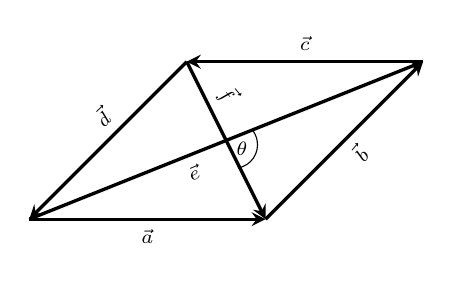
\begin{tikzpicture}[scale=1]
		  \tikzstyle{every node}=[font=\scriptsize]
		  \draw[line width=1.2pt,-stealth](0,0)--(3,0) node[rotate=0,pos=0.5,below]{$\vec{a}$};
		  \draw[line width=1.2pt,-stealth](3,0)--(5,2) node[rotate=50,pos=0.5, below]{$\vec{b}$};
		  \draw[line width=1.2pt,-stealth](5,2)--(2,2) node[rotate=0,pos=0.5, above]{$\vec{c}$};
		  \draw[line width=1.2pt,-stealth](2,2)--(0,0) node[rotate=45,pos=0.45, above]{$\vec{d}$};
		  \draw[line width=1.2pt,-stealth](0,0)--(5,2) node[rotate=23,pos=0.4, below]{$\vec{e}$};
		  \draw[line width=1.2pt,-stealth](2,2)--(3,0) node[rotate=-50,pos=0.3, above]{$\vec{f}$};
		  \draw(2.65,.65) arc (-80:40:.3);
		  \draw(2.7,.9)node[]{$\theta$};
		\end{tikzpicture}
	    \end{center}
	    Así,  $$\cos (\theta) = \dfrac{\vec{e}\circ \vec{f}}{\|\vec{e}\|\|\vec{f}\|} \quad \Rightarrow \quad \theta = \cos^{-1}\left[\dfrac{ (\vec{a}+\vec{b})\circ(\vec{d}+\vec{a})}{\|\vec{e}\|\|\vec{f}\|}\right].$$

	    Luego, ya que $\vec{a},\vec{b},\vec{c},\vec{d}$ forman un rombo. Es decir, un paralelogramo de lados iguales, entonces $\vec{d}=-\vec{b}$, por lo que:
	    $$\theta = \cos^{-1}\left[\dfrac{(\vec{a}+\vec{b})\circ(-\vec{b}+\vec{a})}{\|\vec{e}\|\|\vec{f}\|}\right].$$

	    Por las propiedades de producto interno y $\|\vec{a}\|=\|\vec{b}\|$,

	    $$\begin{array}{rcl}
		\theta&=&\cos^{-1}\left[\dfrac{\vec{a}\circ (-\vec{b})+ \vec{b}\circ(-\vec{b})+ \vec{a}\circ \vec{a}+ \vec{b}\circ \vec{a}}{\|\vec{e}\|\|\vec{f}\|}\right]\\\\
		      &=&\cos^{-1}\left[\dfrac{-(\vec{a}\circ \vec{b})- (\vec{b}\circ \vec{b}) + \vec{a}\circ \vec{a}+ \vec{a}\circ \vec{b}}{\|\vec{e}\|\|\vec{f}\|}\right]\\\\
		      &=&\cos^{-1}\left(\dfrac{ \vec{a}\circ \vec{a}- \vec{b}\circ \vec{b}}{\|\vec{e}\|\|\vec{f}\|}\right)\\\\
		      &=&\cos^{-1}\left(\dfrac{\|\vec{a}\|^2-\|\vec{b}\|^2}{\|\vec{e}\|\|\vec{f}\|}\right)\\\\
		      &=& \cos^{-1}\left(\dfrac{0}{\|\vec{e}\|\|\vec{f}\|}\right) = \dfrac{\pi}{2}.\\\\
	    \end{array}$$
	    Por lo tanto,
	    $$\vec{e}\perp \vec{f}.$$\\

%----------36.
\item 

%----------37.
\item 

%----------38.
\item \textbf{ Demostrar que el segmento que une los puntos medios de dos lados de un triángulo, es paralelo al tercer lado y tiene la mitad de su longitud.\\\\
    Demostración.-}\; Consideremos el siguiente gráfico. Sean $a,b,c,d\in \mathbb{R}^n$ 
	\begin{center}
	    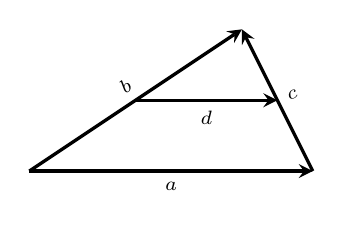
\begin{tikzpicture}[scale=.9]
		\draw[line width=1.2pt,-stealth](0,0)--(4,0) node[rotate=0,pos=0.5, below]{$a$};
		\draw[line width=1.2pt,-stealth](0,0)--(3,2) node[rotate=35,pos=0.5, above]{$b$};
		\draw[line width=1.2pt,-stealth](4,0)--(3,2) node[rotate=20,pos=0.5, right]{$c$};
		\draw[line width=1.2pt,-stealth](1.5,1)--(3.5,1) node[rotate=0,pos=0.5, below]{$d$};
	    \end{tikzpicture}
	\end{center}
	de donde podemos deducir las siguientes ecuaciones:

	$$\left\{\begin{array}{rcl}
		\dfrac{b}{2}-\dfrac{c}{2}-d&=&0\\\\
		a+\dfrac{c}{2}-d-\dfrac{b}{2}&=&0\\
	\end{array}\right. \quad \Rightarrow \quad 
	\left\{\begin{array}{rcl}
		\dfrac{c}{2}&=&\dfrac{b}{2}-a\\\\
		\dfrac{c}{2}&=&d+\dfrac{b}{2}-a\\\\
	\end{array}\right.$$

	Entonces $a=2d$ si y sólo si $a \parallel d$. Así tomando la norma nos queda:
	$$\|a\|=\|2d\| \quad \Rightarrow \quad \|d\|=\dfrac{1}{2}\|a\|.$$\\

%----------39.
\item

%----------40.
\item 

%----------41.
\item \textbf{\boldmath Demostrar vectorialmente la ley de cosenos.\\\\
    Demostración.-}\; Supongamos que $\vec{a},\vec{b} \in V_n$ y, 
    \begin{center}
	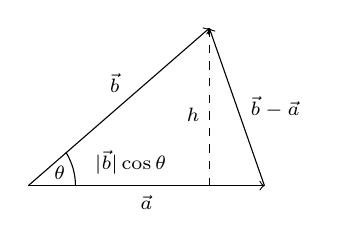
\begin{tikzpicture}
	    \draw[->](0,0)--(3,0);
	    \draw(1.5,0)node[below]{$\vec{a}$};
	    \draw[->](3,0)--(2.3,2);
	    \draw(1.1,1.3)node[]{$\vec{b}$};
	    \draw[<-](2.3,2)--(0,0);
	    \draw(2.7,1)node[right]{$\vec{b}-\vec{a}$};
	    \draw[dashed](2.3,2)--(2.3,0);
	    \draw(1.3,.3)node[]{$|\vec{b}|\cos \theta$};
	    \draw(2.3,.9)node[left]{$h$};
	    \draw(.4,.17)node[]{$\theta$};
	    \draw (0:.6cm) arc (0:32:.8cm);
	\end{tikzpicture}
    \end{center}
    entonces por el teorema de Pitágoras se tiene $$h^2=|\vec{b}|^2 - \left(|\vec{b}|\cos \theta\right)^2 \qquad y \qquad |\vec{b}-\vec{a}|^2 = \left(|\vec{b}|\cos \theta - |\vec{a}|\right)^2+h^2$$
    de donde $$|\vec{b}-\vec{a}|^2 = \left(|\vec{b}|\cos \theta - |\vec{a}|\right)^2+|\vec{b}|^2 - \left(|\vec{b}|\cos \theta\right)^2 = \left(|\vec{b}|\cos \theta\right)^2 - 2|\vec{a}||\vec{b}|\cos \theta + |\vec{a}|^2 + |\vec{b}|^2 - \left(|\vec{b}|\cos \theta\right)^2$$
    por lo tanto, $$|\vec{b}-\vec{a}|^2 = |\vec{a}|^2 + |\vec{b}|^2 - 2|\vec{a}||\vec{b}|\cos \theta $$\\

%----------42.
\item 

\end{enumerate}


